\documentclass{standalone}
\usepackage{graphicx}	
\usepackage{amssymb, amsmath}
\usepackage{color}

\usepackage{tikz}
\usetikzlibrary{shapes}
\usepackage{pgfmath}

\definecolor{light}{RGB}{220, 188, 188}
\definecolor{mid}{RGB}{185, 124, 124}
\definecolor{dark}{RGB}{143, 39, 39}
\definecolor{highlight}{RGB}{180, 31, 180}
\definecolor{gray10}{gray}{0.1}
\definecolor{gray20}{gray}{0.2}
\definecolor{gray30}{gray}{0.3}
\definecolor{gray40}{gray}{0.4}
\definecolor{gray60}{gray}{0.6}
\definecolor{gray70}{gray}{0.7}
\definecolor{gray80}{gray}{0.8}
\definecolor{gray90}{gray}{0.9}
\definecolor{gray95}{gray}{0.95}

\newcommand*{\h}{40}

\begin{document}

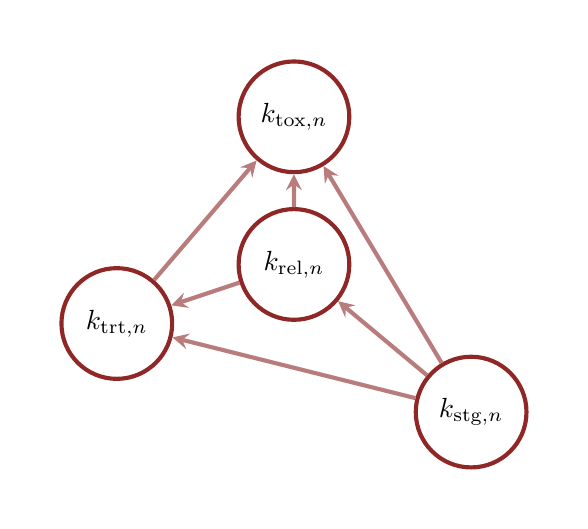
\begin{tikzpicture}[
   scale=0.2,
   obscirc/.style={circle, draw=dark, fill=dark, line width=1.5, text=white,
               inner sep=5, minimum size=\h},
   obsell/.style={ellipse, draw=dark, fill=dark, line width=1.5, text=white,
                  inner sep=5, minimum height=\h},
   obsrec/.style={rectangle, draw=dark, fill=dark, line width=1.5, text=white,
                  inner sep=5, minimum height=\h, minimum width=27},
   unobscirc/.style={circle, draw=dark, fill=white, line width=1.5, text=black,
                     inner sep=5, minimum size=\h},
   unobsell/.style={ellipse, draw=dark, fill=white, line width=1.5, text=black,
                    inner sep=1, minimum height=\h},
   unobsrec/.style={rectangle, draw=dark, fill=white, line width=1.5, text=black,
                    inner sep=1, minimum height=\h, minimum width=27},
   pushcirc/.style={circle, draw=dark, fill=white, line width=1.5, dashed, text=black,
                    inner sep=1, minimum size=\h},
   pushell/.style={ellipse, draw=dark, fill=white, line width=1.5, dashed, text=black,
                   inner sep=1, minimum height=\h}
  ]

  % Node Spacing
  \pgfmathsetmacro{\d}{7.5}
  
  \begin{scope}[shift={(0, 0)}]
    \draw[white] (-6.75 * \d, -5.25 * \d) rectangle (-2.25 * \d, -1.25 * \d);

    %\node (A) at (0, -6 * \d) [unobscirc] { $q_{C_{0}}$ };

    %\node[anchor=west] at (1.1 * \d, -1 * \d) { $p(q_{C_{0}}) = \text{beta}(q_{C_{0}} \mid 12.7, 3.7)$ };
    
    %\node (B) at (0, 0.5 * \d) [pushcirc] { $q_{C, n}$ };
    
    %\node (C) at (1.5 * \d, -6 * \d) [unobscirc] { $q_{AC}$ };

    %\node (D) at (1.5 * \d, 1.25 * \d) [pushell] { $q_{NC + AC, n}$ };

    %\node (E) at (0, 3 * \d) [unobscirc] { $y_{n}$ };
    
    %\node (F) at (-1.5 * \d, 1.75 * \d) [pushcirc] { $\alpha_{\text{tox}, n}$ };
    %\node (G) at (-1.5 * \d, 0.5 * \d) [pushcirc] { $\alpha_{\text{rel}, n}$ };
    %\node (H) at (-1.5 * \d, -0.75 * \d) [pushcirc] { $\alpha_{\text{stg}, n}$ };

    %\node (I) at (-7.5 * \d, 1.75 * \d) [unobscirc] { $\boldsymbol{\alpha}_{\text{tox}}$ };
    %\node (J) at (-7.5 * \d, 0.5 * \d) [unobscirc] { $\boldsymbol{\alpha}_{\text{rel}}$ };
    %\node (K) at (-7.5 * \d, -0.75 * \d) [unobscirc] { $\boldsymbol{\alpha}_{\text{stg}}$ };


    \node (L) at (-4.5 * \d, -2 * \d) [unobscirc] { $k_{\text{tox}, n}$ };
    \node (M) at (-6 * \d, -3.75 * \d) [unobscirc] { $k_{\text{trt}, n}$ };
    \node (N) at (-4.5 * \d, -3.25 * \d) [unobscirc] { $k_{\text{rel}, n}$ };
    \node (O) at (-3 * \d, -4.5 * \d) [unobscirc] { $k_{\text{stg}, n}$ };
    
    %\node[anchor=west] at (1.1 * \d, 2.25 * \d) { $p( y_{1}, \ldots, y_{N} \mid q_{C_{0}}, \boldsymbol{\alpha})$ };
    %\node[anchor=west] at (1.1 * \d, 1.75 * \d) { $\quad= \prod_{n = 1}^{N} \text{Bernoulli}( y_{n} \mid q_{n} )$ };
    
    
    %\node (D) at (-2 * \d, 0 * \d) [unobscirc] { $\boldsymbol{\alpha}_{\text{rel}}$ };
    %\node (E) at (-2 * \d, 0.5 * \d) [unobscirc] { $\boldsymbol{\alpha}_{\text{stg}}$ };
    %\node (F) at (-2 * \d, 1 * \d) [unobscirc] { $\boldsymbol{\alpha}_{\text{tox}}$ };
    
    
    %\draw[dark, line width=1.5, rounded corners=2] (-6.75 * \d, {-5.25 * \d}) rectangle (3 * \d, 3.75 * \d);

    \foreach \B/\E in {O/L, O/M, O/N, N/L, N/M, M/L} {
      \draw[->, >=stealth, color=mid, line width=1.5] (\B) -- (\E);
    }

  \end{scope}

\end{tikzpicture}

\end{document}  